\section{Metodolog\'ia}

\subsection{Tipo de Investigaci\'on}
La investigaci\'on es de tipo experimental y comparativa. Se implementan modelos cu\'anticos y cl\'asicos bajo condiciones controladas, variando sistem\'aticamente los componentes del circuito cu\'antico para analizar su impacto en el rendimiento.

\subsection{Datasets}

\subsubsection{Dataset Iris}
El dataset principal es Iris de Fisher, que contiene 150 muestras con 4 caracter\'isticas num\'ericas (longitud y ancho de s\'epalo y p\'etalo) y 3 clases (setosa, versicolor, virginica) con 50 muestras cada una. Las caracter\'isticas fueron normalizadas al rango $[0, \pi]$ para permitir la codificaci\'on angular en puertas de rotaci\'on cu\'anticas.

\subsubsection{Dataset MNIST Reducido}
Como experimento secundario, se utiliz\'o el dataset digits de scikit-learn, filtrado a las clases 0 y 1 (360 muestras). Se aplic\'o PCA para reducir de 64 a 4 componentes, normalizando al rango $[0, \pi]$.

\subsection{Preprocesamiento}
\begin{enumerate}
    \item Normalizaci\'on MinMaxScaler al rango $[0, \pi]$ para codificaci\'on angular.
    \item One-hot encoding de las etiquetas (requerido por VQC).
    \item Split estratificado 70/30 con semilla fija (42) para reproducibilidad.
\end{enumerate}

\subsection{Modelos Implementados}

\subsubsection{Modelos Cl\'asicos (Baselines)}
Se implementaron con scikit-learn:
\begin{itemize}
    \item \textbf{SVM-RBF}: kernel RBF, $C=1.0$, $\gamma=$scale.
    \item \textbf{MLP}: capas ocultas (16, 8), 2000 iteraciones m\'aximas.
    \item \textbf{KNN}: $k=5$ vecinos.
\end{itemize}

\subsubsection{Modelos Cu\'anticos}
Se implementaron con Qiskit Machine Learning 0.9.0:
\begin{itemize}
    \item \textbf{VQC}: ZZFeatureMap (reps=2, linear) + RealAmplitudes (reps=3, linear) + COBYLA (200 iteraciones). Funci\'on de costo: entrop\'ia cruzada. Primitiva: StatevectorSampler.
    \item \textbf{QSVC}: FidelityQuantumKernel con ZZFeatureMap (reps=2, linear), delegando a SVC de scikit-learn.
\end{itemize}

\subsection{Dise\~no del Circuito Cu\'antico}
El circuito completo utiliza 4 qubits (uno por caracter\'istica). El feature map ZZFeatureMap codifica las caracter\'isticas mediante rotaciones $R_Z$ e interacciones $R_{ZZ}$ con entrelazamiento lineal. El ansatz RealAmplitudes a\~nade 16 par\'ametros entrenables distribuidos en 3 capas de rotaciones $R_Y$ y CNOT.

\begin{figure}[h]
\centering
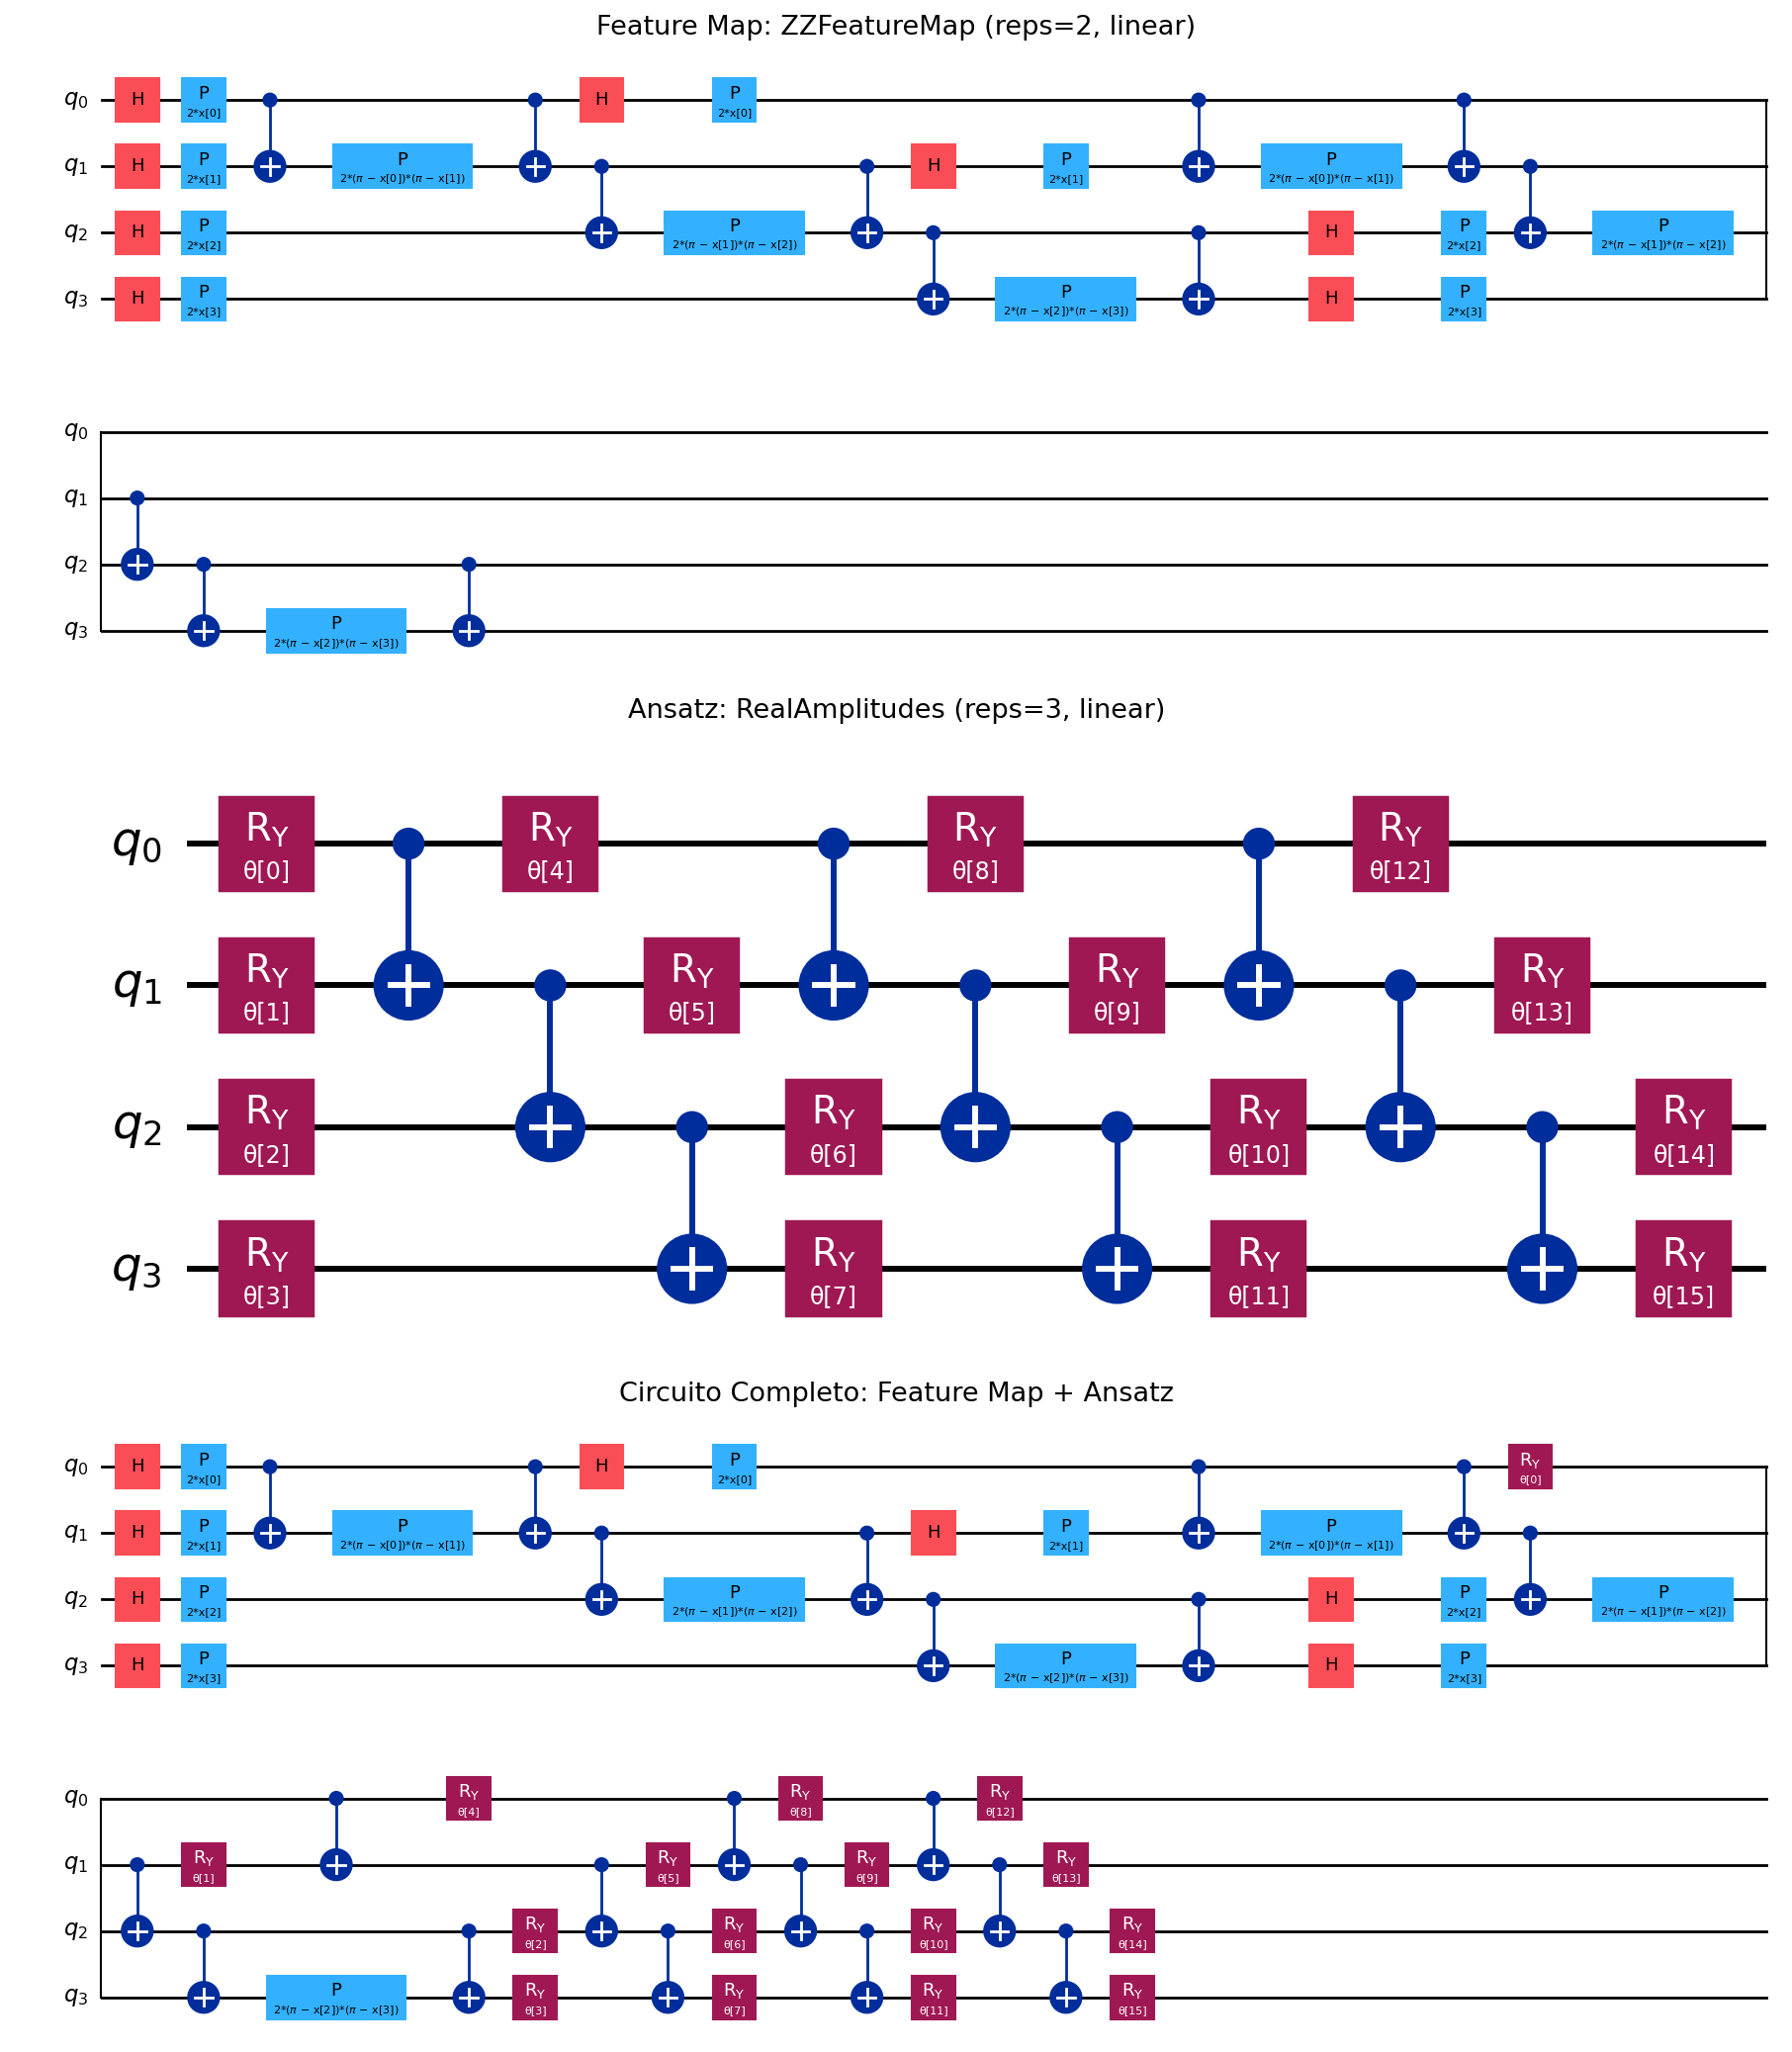
\includegraphics[width=\textwidth]{figuras/circuitos.png}
\caption[Circuitos cu\'anticos utilizados]{Arriba: ZZFeatureMap (reps=2). Centro: RealAmplitudes (reps=3). Abajo: circuito completo.}
\label{fig:circuitos}
\end{figure}

\subsection{Experimentos Realizados}
\begin{enumerate}
    \item \textbf{Comparaci\'on feature maps}: ZFeatureMap, ZZFeatureMap (linear), ZZFeatureMap (full), PauliFeatureMap.
    \item \textbf{Profundidad del ansatz}: reps $\in \{1, 2, 3, 5\}$ en RealAmplitudes.
    \item \textbf{Optimizadores}: COBYLA, SPSA, L-BFGS-B.
    \item \textbf{Varianza}: VQC ejecutado con 5 semillas distintas.
    \item \textbf{Ruido NISQ}: perturbaci\'on gaussiana con $\sigma \in \{0, 0.05, 0.10, 0.20, 0.30, 0.50\}$.
    \item \textbf{Generalizaci\'on}: evaluaci\'on en MNIST reducido (clases 0 vs 1).
\end{enumerate}

\subsection{M\'etricas de Evaluaci\'on}
\begin{itemize}
    \item Accuracy, Precision (macro), Recall (macro), F1-Score (macro).
    \item Tiempo de entrenamiento.
    \item Curvas de convergencia (loss vs iteraci\'on).
    \item Matrices de confusi\'on.
    \item Validaci\'on cruzada 5-fold para modelos cl\'asicos.
\end{itemize}

\subsection{Herramientas}
\begin{itemize}
    \item Python 3.11, Qiskit 2.4.1, Qiskit Machine Learning 0.9.0.
    \item scikit-learn, NumPy, Matplotlib, Pandas.
    \item Simulaci\'on con StatevectorSampler (sin ruido de hardware).
\end{itemize}
